\section{Grundlagen}\label{sec:grundlagen}
Dieses Kapitel soll einen grundlegenden Überblick über die zwei wichtigsten Themengebiet dieser Arbeit bieten, Schule und IT und der damit verbundene Einsatz von digitalen Unterrichtsmethodiken
\subsection{Digitalisierung an Schulen}\label{sec:digianschulen}
Die folgenden zwei Abschnitte sollen einen Einblick und eine Momentaufnahme über den Stand der Digitalisierung an deutschen Schulen (Stand 2018/2019) und den möglichen Potential von digital gestützten interaktiven Unterrichtsmethoden bieten. Ebenso wird das Thema Datenschutz an Schulen näher betrachtet.

\subsubsection{Momentaufnahme}\label{sec:technikunterricht}
Laut einer aktuellen Studie von Citrix, sind deutsche Schüler mit Abstand am schlechtesten 
ausgestattet, was Technologie im Unterricht angeht\cite{Technisc27:online}. Die Studie hat dabei einen direkten Vergleich zwischen den vier europäischen Ländern Frankreich, Großbritannien, Niederlande und Deutschland gezogen und pro Land mehr als 1000 Schülerinnen und Schüler befragt (Niederlande 500). 22\% gaben an, gar keine Technologie im Unterricht einzusetzen, die über das Anzeigemedium Projektor hinausgeht. Innovative Technologien wie der im Abschnitt \ref{sec:zielsetzung} erwähnte Einplantinencomputer Raspberry Pi, mit denen u.A. IoT-Projekte umgesetzt werden können, stehe nur 13\% der Schülerinnen und Schülern an deutschen Schulen zur Verfügung. \\ 
Oftmals ist der normale Zustand an einer Schule jener, dass ein IT-interessierter Lehrender oder sogar die Hausmeisterin/der Hausmeister selbst, administrative Aufgaben die Schul-IT betreffend übernimmt, was an einem Fachpersonalmangel festzumachen sei, so Ralf Koenzen, Gründer und Geschäftsführer der LANCOM Systems GmbH im Fachartartikel 'IT-Infrastrukturen an Schulen: Von der Kreidezeit ins digitale Zeitalter'\cite{Koenzen2018}. Darüber hinaus seien funktionstüchtige Projektoren und Computer vielerorts Mangelware ebenso das Funknetzwerk (WLAN) nur begrenzt, wenn überhaupt, verfügbar. 

\begin{figure}[H]
	\centering
	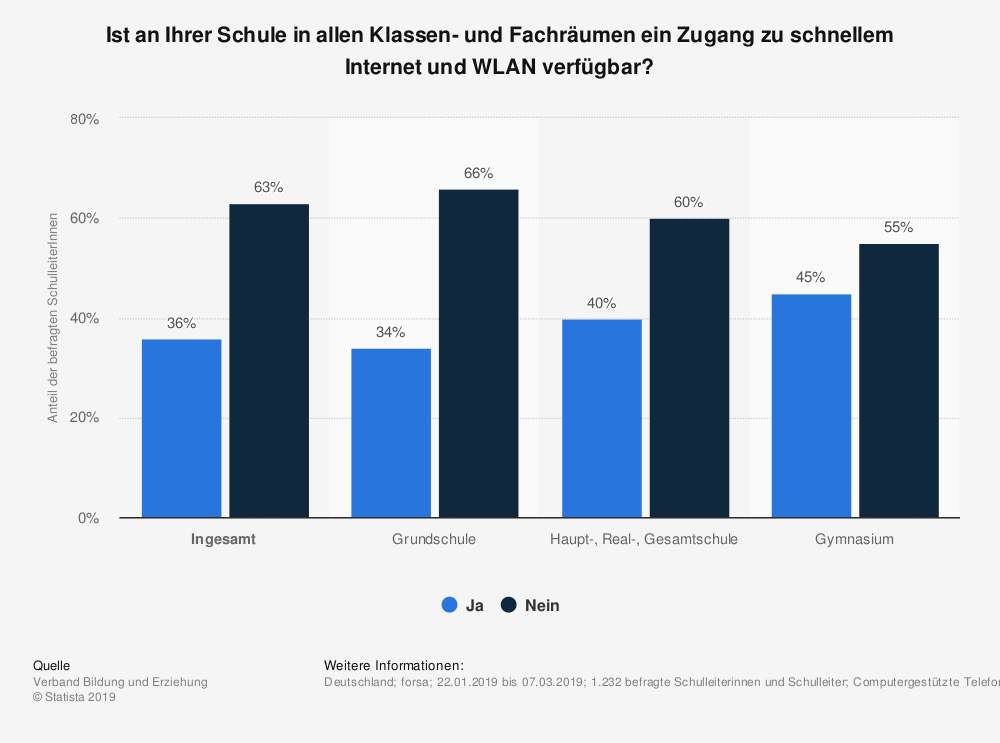
\includegraphics[width=0.8\linewidth]{bilder/statista_wlan}
	\caption[Verfügbarkeit von schnellem Internet und WLAN in Klassenräumen]{Verfügbarkeit von schnellem Internet und WLAN in Klassenräumen: Bundesweiten Erhebung zum Thema Digitalisierung an allgemeinbildenden Schulen in Deutschland. \cite{VBE2019}}
	\label{fig:statistawlan}
\end{figure}


Allerdings scheinen die ersten Barrieren durch den, in der  \hyperref[sec:einleitung]{Einleitung} dieser Arbeit bereits erwähnten, Digitalpakt Schule zu fallen. Dieser sieht vor fünf Millarden Euro in die IT-Ausstattung der deutschen Schulen fliesen zu lassen. Eine Schule mit mehr als tausend Schülern und entsprechendem Lehrkörper steht der Anforderungskomplexität an IT-Systeme eines größeren Wirtschaftsunternehmen kaum nach. Eine Ausnahme bilden hier Schulen, die auf professionelle Betreuung durch ein Systemhaus oder eigene Netzwerktechniker setzen\cite{Koenzen2018}. \\ \\ Eine interessante Alternative könnte hier das Nutzen von Cloud-Technologie sein. Cloud-basierte Netzwerkmanagementlösungen und Software-defined Networking (SDN) scheint im Wirtschaftssektor bereits auf dem Vormarsch zu sein. Diese Technologien könnte Schulen dabei unterstützen den Digitalisierungsfortschritt voranzutreiben. Hierbei werden notwendige infrastrukturelle Geräte wie Access Points, Router, Switches und die nötige Verkabelung direkt vor Ort in der Schule installiert. Die Betreuung und Wartung erfolgt jedoch höchstmöglich automatisiert mit geringerem Aufwand aus der Ferne. 



\subsubsection{Ausblick digital gestützte interaktive Unterrichtsmethoden}\label{sec:interaktiveunterr}
Die erwähnte Technik im Abschnitt \ref{sec:digianschulen} macht den Einsatz von digital gestützten Interaktiven Unterrichtsmethoden möglich. Der online Lernvideo Anbieter Sofatutor hat im Jahr 2016 auf dem Educamp Leipzig Lehrerinnen und Lehrer über Software befragt, welche diese erfolgreich in ihren Unterricht integriert haben\cite{Sofatutor2019}. Neben zahlreicher Software, welche der Unterrichtsvorbereitung dient, lässt eine umfangreiche Liste in der Sektion 'Interaktion' finden. Zum Beispiel lassen sich verschiedene Aufgabenformen ausmachen, die dann an einer digitalen Tafel von den Schülerinnen und Schülern gelöst werden sollen. Dies umfasst z.B. das Markieren, Sortieren, Zuordnen (Paare finden) von Bildern, Multiple Choice Aufgaben, Quiz Anwendungen, App-gestützte Spiele wie interaktive Lern-Rallyes (Rätsel, Herausforderungen und Medieninhalte können vielfältig miteinander verbunden werden), Brainstorming, u.v.m. Generell lässt sich feststellen, dass die Palette von Anwendungsmöglichkeiten enorm ist und viele klassische Konzepte, die sich bereits analog interaktiv durchführen lassen konnten, auch in einer digitalen Version bereitstehen. Beispielsweise können Unterrichtsmethoden wie ein Lern-Quiz sich auch mit Papier und Stiften durchführen, digitale Technik kann hier jedoch viel Arbeit abnehmen und lässt die Ausführung der Unterrichtsmethodik deutlich immersiver und medial interaktiver zu. So kann das Medium Film eingebettet werden, was analog nur sehr aufwändig möglich wäre. Abseits spielerischer Szenarien lässt die Mathematik Software GeoGebra das visualisieren von mathematischen Zusammenhängen zu. So können diese visualisiert und die Auswirkung von anderen Werten gezeigt werden. Das Konzept Bring-your-own-device, welches vorsieht das zu Unterrichtende eigene Geräte mitbringen, wie z.B. ein Smartphone, steigert das Maß von Interaktivität zusätzlich. So ist es möglich, dass eine ganze Lerngruppe oder gänzliche Schulklasse simultan einer interaktiven Unterrichtsmethode partizipiert. Ebenso kann ein Dozierender in einer Prüfungssituation auf Software zurückgreifen, welche die Prüfung des Kandidat unterstützt und eine anschließende Auswertung der Antworten wesentlich automatisiert und vereinfacht. An vielen deutschen Universitäten, wie auch der HTW Berlin, wird die Software Moodle für diesen Zweck eingesetzt. Zusammenfassend lässt sich feststellen, dass das Potential von digital gestützten Unterrichtsmethoden deutlich gegeben und das Angebot sowie Möglichkeiten der Anwendungen enorm ist. Eine bewusste Einbettung in den Unterricht kann ebendiesen positiv unterstütze und den Lehrenden entlasten. Als positiven Nebeneffekt lässt sich das Steigern von digitalen Kompetenzen seitens der Schülerinnen und Schülern vermerken, welche im Zuge der immer fortschreitenden Digitalisierung weltweit eine nicht zu unterschätzende Fähigkeit ist. 

\subsubsection{Datenschutz an Schulen}\label{sec:datenschutz}
Am 25. Mai 2018 gilt die neue EU-Datenschutzverordnung, welche für alle Personen, Behörden oder sonstigen Stellen anzuwenden ist, wenn personenbezogene Daten verarbeitet werden. Dies betrifft also auch Schulen. Dies ist sofern nichts neues, da die Datenverarbeitung und Auskunftsrechte in §64 des SchulG (Schulgesetz) im Falle des Bundeslands Berlin geregelt sind und dieser weiterhin anzuwenden ist. Neu ist allerdings, dass die Verantwortlichen für die Verarbeitung von personenbezogenen Daten weitere Aspekte müssen, welche die neue Datenschutzverordnung mit sich bringt. Weiterführend sei hierzu die Quelle \cite[Datenschutz in der Schule]{Kachelriess2019} zu nennen. In diesem Zusammenhang ist es wichtig, dass auch eingesetzte Software an Schulen zu diesen Bestimmungen kompatibel sein muss, wenn diese personenbezogene Daten verarbeitet. Im Jahr 2018 an der Düsseldorfer Gemeinschaftsschule haben Unklarheiten um den Schutz von Schülerdaten dafür gesorgt, dass die Zeugnisse der rund 300 Schülerinnen und Schüler wieder per Hand geschrieben wurden. Auch die im vorherigen Abschnitt genannten Bring-your-own-device Praxis befindet sich Stand 2018 noch in einer rechtlichen Grauzone, sollten personenbezogene Daten verarbeitet werden\cite{WitmerGossner2018}. Die im Abschnitt \ref{sec:technikunterricht} genannte Auslagerung in eine Cloud könnte hier ebenfalls helfen, wenn der Cloud-Anbieter EU-Datenschutzverordnung konform arbeitet. Es ist auf jeden Fall ratsam, wenn Cloud-Anbieter und Server ihren Standort in Deutschland haben.

\newpage

\subsection{Überblick Webtechnologie}\label{sec:webbasedsoftware}
% Hier auf PDF Technische Anforderungen verweisen (Footnote?) da sehr ausführlich und gut
% Anfang Geschichtlich
Diese Sektion soll einen grundlegenden über im Kontext dieser Arbeit wichtigen Begrifflichkeiten bieten. Die folgenden Untersektion 2.2.1 ff. werden die Thematiken nur grob umreißen, da eine detaillierte Betrachtung der genannten Begriffe den Rahmen dieser Arbeit weit überschreiten würde. 

\subsubsection{Intranet und Internet}\label{sec:intranetundinternet}
% Detailgrad so sinnvoll?
% Unterschied und Gemeinsamkeit klar machen
% Hier kommunikation erklären! Protokolle und OSI schicht!
Einfach ausgedrückt, ist das Internet ein Netzwerk von Computern, welche weltweit miteinander vernetzt sind. Seine Anfänge lassen sich auf das Ende der 1960er in den USA datieren, als die DARPA (Defense Advanced Research Projects Agency) eine weltweite Verknüpfung von Datennetzen anstrebte. Das hier draus resultierende ARPANET (Advanced Research Projects) kann als Ursprung angesehen werden. Dabei beschreibt der Begriff Internet streng genommen ein 'interconnected network', also ein international vernetztes Netzwerk, ohne dabei die Hardware- und Netzwerktechnologie genauer zu beschreiben \cite{Safran2011}.  \\ 
Der wohl populärste Anwendung des Internets ist das World Wide Web, welche gegen das Jahr 1989 von einer Forschungsgruppe rund um Sir Tim Berners-Lee ins Leben gerufen wurde und heute oftmals als Synonym für das gesamte Internet sprachlich genutzt wird. \\ 

In unser heutigen globalisierten Welt lässt sich das Internet mitsamt World Wide Web nicht mehr wegdenken und ist ein integraler Bestandteil der Informationskultur. 
 \\ \\
 Das Intranet beschreibt analog dazu ein lokal abgeschlossenes Netzwerk von Computern, bspw. innerhalb eines Unternehmens. Dabei endet ein Intranet klar an seinen Grenzen und ein Gateway fungiert als Übergabepunkt ins Internet. Die Vernetzung der Endgeräte erfolgt kabelgebunden (LAN) oder kabellos (WLAN). Die Kommunikationsgeschwindigkeit innerhalb eines Intranets sind i.d.R. deutlich höher als im Internet, da Daten nicht erst nach außen an einen Internet Service Provider übermittelt werden müssen. Ein Intranet funktioniert unabhängig vom öffentlichem Internet (erhöhte Ausfallsicherheit), ist nicht öffentlich zugänglich und bietet oft andere oder zusätzliche Funktionen. \cite{Intranet62:online}. 
 
 \subsubsection{Client-Server Modell}\label{sec:clientservermodell}
 Das Client-Server Modell beschreibt das Prinzip der Kommunikation zwischen zwei Teilnehmer innerhalb eines Netzwerks. Grundlegend unterscheidet das Modell hierbei zwischen einer Anbieterseite (Server) und einer Benutzerseite (Client). Der Client betreibt auf seinem Endgerät (Computer, Smartphone, etc.) eine Clientsoftware mit der die Verbindung zum Server aufgebaut wird. Im Fall des WWW (siehe \ref{sec:www}) ist dies in den meisten Anwendungsszenarien ein Webbrowser. Der Client fordert dabei eine Resource an, welche auf dem Server vorliegt oder dort speziell für die Anfrage des Clients generiert wird (siehe auch Sektion \ref{sec:webanwenservices}). Das Client-Server Modell sieht vor, dass immer der Client die Verbindung aufbaut, nie andersherum \cite{ElektronikKompendium.de:online}. Die Anfrage des Clients wird Request genannt, die Antwort des Servers Response oder Reply, welche bei ausreichender Berechtigung des Clients auch Daten enthält. 
 Server-Computer sollen rund um die Uhr erreichbar sein, während Client-Endgeräte auch abgeschaltet werden können, ohne die Integrität des Netzwerks zu beeinflussen. 
  % Vergleich zu anderen Modellen?
 
\subsubsection{Kommunikation}\label{sec:kommunikation}
Die Kommunikation im Internet und Intranet erfolgt über Protokolle. 
Ein Protokoll kann als ein Satz von Kommunikationsregelvorschriften verstanden werden \cite{Safran2011}, welche den Netzwerkverkehr auf unterschiedlichen Schichten reglementieren. 
Diese Schichten werden im OSI-Modell (Open System Interconnection) der ISO (International Standardization Organisation), der internationalen Standardisierungsorganisation beschrieben. (Siehe Tabelle) %HIER TABELLE!
\\ 
Das OSI-Modell ist dabei in sieben Schichten eingeteilt, während die Erste als physikalische Schicht definiert ist und die Siebte als Anwendungsschicht. Protokolle sind dabei jeweils nur über Protokolle benachbarter Schichten in Kenntnis gesetzt. Das OSI-Modell lässt sich grob in anwendungsorientierte Schichten (1 bis 4) und transportorientierte Schichten (5 bis 7) unterteilen. Die im Rahmen dieser Arbeit genutzten Webtechnologien nutzen kommunikativ nur anwendungsorientierte Schichten des ISO-OSI Modells.



% Begriff Internet
\subsubsection{World Wide Web}\label{sec:www}
Das World Wide Web (WWW) ist die wohl populärste Anwendung des Internets \cite{Safran2011} und wird oftmals fälschlicherweise als Synonym für das gesamte Internet genannt. Das WWW ist eine Sammlung von verteilten Dokumenten, welche sich gegenseitig über sog. Hyperlinks referenzieren und von Web-Servern zur Verfügung gestellt werden. Auf der Client Seite (siehe \ref{sec:clientservermodell}) stellt der Web-Browser die wichtigste Software da. Mit ihr werden Web Server angesprochen (Request) und Antworten (Response) für den Nutzenden dargestellt. Die wichtigsten sprachlichen Komponenten des WWW sind: \\ 
\begin{itemize}
	\item HTML: Hypertext Markup Language - eine reine Beschreibungssprache, welche Hypertext Dokumente durch Tags codiert. 
	\item CSS: Cascading Style Sheet - Eine Stylesheet Sprache, welche das äußere Erscheinungsbild von Hypertext Dokumenten beschreibt
	\item JS: JavaScript: Eine Skriptsprache, welche u.A. Interaktion sowie Dynamik hinzufügt und clientseitig interpretiert wird. 
\end{itemize}
Die Techniken des WWW können auch lokal im Intranet genutzt werden. 
Das zur Verständigung zwischen Client und Server genutzte Protokoll (siehe \ref{sec:kommunikation})ist das Hypertext Transfer Protocol (HTTP) bzw. in verschlüsselter Form Hypertext Transfer Protocol Secure, da eine Übermittlung im Klartext nicht immer wünschenswert ist. HTTP/HTTPS ist ein Zustandsloses Protokoll, das bedeutet dass jede Anfrage unabhängig voneinander geschieht und betrachtet wird. Dies und die Tatsache, dass jede Anfrage von der Client-Seite aus gestartet werden muss (siehe \ref{sec:clientservermodell}), stellen oftmals Hürden für die Entwicklung von Webanwendungen und Webservices da. Techniken wie Cookies und Sessions, sowie das wiederholte Abfragen von aktualisierten Daten seitens des Clients wirken hier entgegen. Cookies stellen persistent gespeicherte Daten auf der Client-Seite da, mit deren Hilfe der Webserver einen Client eindeutig zuordnen kann. Bei einer Session sendet der Client bei jeder Anfrage eine eindeutige ID an den Server. Im Normalfall endet eine Session beim Beenden des Webbrowser, während Cookie-Dateien eine längere Lebensdauer besitzen.      
%
\subsubsection{Webanwendungen und Webservices}\label{sec:webanwenservices}
Im Laufe der Entwicklung des WWW (\ref{sec:www}) stieg der Anspruch vom reinen Anbieten statischer Dokumenten in Richtung dynamischer Inhalte, welche einer Programmlogik folgend von einem Webserver für jede Anfrage generiert werden. Webanwendungen sind Computerprogramme, welche auf einem Webserver ausgeführt werden und den Webbrowser des Clients als Schnittstelle nutzen \cite{Safran2011}. Dies bietet den großen Vorteil, dass etwaige Anpassungen von Programmlogik nur serverseitig erfolgen müssen und jeder Client mit Webbrowser als Benutzerschnittstelle ausreicht. \\ \\
Webservices sind eine spezialisierte Art von Webanwendung. Die Fokus hier liegt auf das bereitstellen von Daten für andere Applikationen, welche die gewonnen Daten selbst auswerten und dem Nutzenden bereitstellen. Dies geschieht i.d.R. über eine einheitlich beschriebene Schnittstelle (API - Application Programming Interface), über welche fremde Applikationen angefragte Daten abrufen können. Der Austausch der Daten erfolgt hier meist über Formate wie JSON (JavaScript Object Notation) oder XML (Extensible Markup Language), da Aussehen und Lesbarkeit der Daten irrelevant sind und somit eine Ausgabe in HTML nicht von Nöten ist. \\
Bei der Implementierung eines Webservices bieten sich folgende zwei technologische Arten der Umsetzung an: \\ \\
\textbf{SOAP/WSDL}: Hier werden Nachrichten über das Simple Object Access Protocoll ausgetauscht (SOAP) und deren Beschreibung über die Web Services Description Language (WSDL) definiert. Anfrage- und Antwortformat der Daten ist XML (Extensible Markup Language), eine Auszeichnungssprache, welche HTML sehr ähnelt aber deutlich allgemeiner ist. XML kann als mehr als Regelwerk verstanden werden, mitdessen Hilfe Entwickler ihre eigene hierarische Beschreibung einer Datenstruktur vornehmen können. XML und HTML leiten sich bei der von der SGML (Standard Generalized Markup Language) ab, welches ihre Ähnlichkeit zusätzlich herleitet \cite{XMLHTMLU88:online}. \\

 
\textbf{REST}: (Representational State Tranfer) Hier kann jede einzelne Funktion des Webservices über eine jeweils zugeordnete URL abgerufen (Uniform Resource Locator) werden, umgangssprachlich als Webadresse bekannt. Das WWW selbst kann als REST-Webservice verstanden werden \cite{Bayer2002:online}. \\ 

\subsection{Websockets}\label{sec:websockets}
Bezugnehmend auf die Problematik, welche durch die Kommunikationsstrategie über das http-Protokoll entsteht (siehe Sektion \ref{sec:www}), wirken Websockets dieser entgegen. Als Kommunikationskanal verknüpft ein Websocket Server und Client. Zwar muss die Kommunikation zunächst über den Client initiiert werden, bleibt dann jedoch bestehen und der Server kann diese nutzen um aktiv neue Daten zu emittieren. Ein Nachteil ist jedoch, dass im Gegensatz zum http-Protokoll hier auch Daten hin- und hergeschickt werden, wenn dies eventuell nicht gewünscht ist \cite{neumann2015entwicklung}, was insbesondere bei mobilen Applikationen kritisch sein kann. Ein generellen Vorteil bieten Websockets auch in Sachen Performanz, da das Protokoll, ist erst einmal eine Verbindung zustande gekommen, deutlich schlanker ist. \\ Das folgende Bild zeigt einen Performanz Vergleich in Anbetracht des zusätzlichen Payloads von REST- und WebSocket Nachrichten. 

\begin{figure}[H]
	\centering
	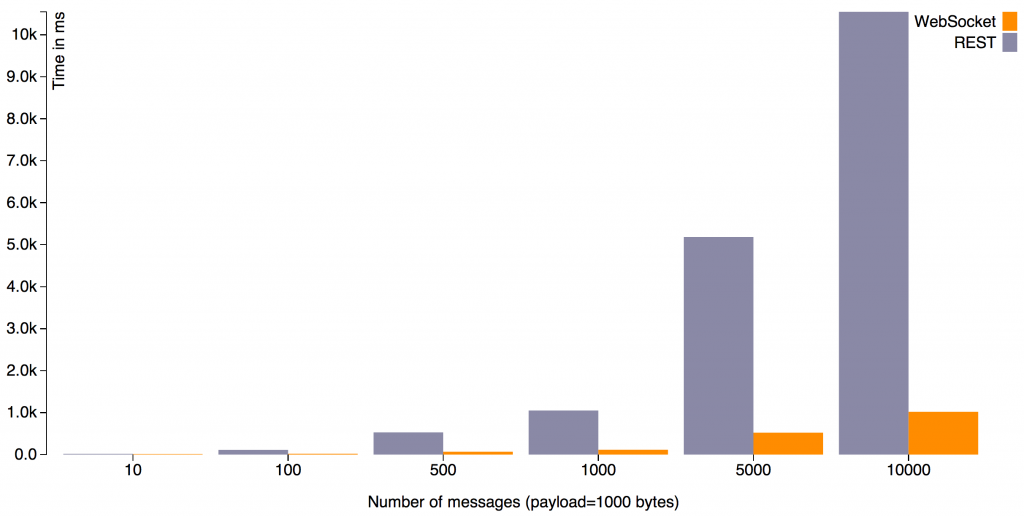
\includegraphics[width=0.8\linewidth]{bilder/websocket-rest-messages}
	\caption[Performanzvergleich REST versus WebSockets]{Performanzvergleich REST versus WebSockets - Benötigte Zeit um N Nachrichten einer konstanten Nachrichtengröße zu verarbeiten. \cite{Gupta2014}}
	\label{fig:socketsrest}
\end{figure}

\subsection{Webapplikationsentwicklung}\label{sec:softwareentwicklung}
Dieses Kapitel soll den wesentlicheren Bestandteil dieser Arbeit grundlegend beleuchten, der Entwicklung von Webapplikationen.
Webanwendungen und Webservices können unter diesem Begriff zusammengefasst werden.
 \\ 
\subsubsection{Web-Application-Frameworks} \label{sec:wafs}
Bei der Entwicklung von Webapplikationen wird oftmals auf Frameworks (z.Dt. Rahmengerüste), spezifischer Web-Application-Framework (WAF) zurückgegriffen. 
Ein WAF bezeichnet damit ein Programmgrundgerüst, welches als Grundlage zum Einsatz kommt \cite{Ionis2019:online}. Dies erleichtert die Entwicklung ungemein, da auf bereits vorgefertigte Ansätze und Programmbausteine zugegriffen werden kann und diese nicht selbst von Hand implementiert werden müssen. Diese WAFs reflektieren zumeist auch eine Modelle und Prinzipien, welche, falls dem Entwickelnden bekannt, den Einstieg erleichtern. 
Ein für Frameworks bekanntes Paradigma stellt das Umsetzungsparadigma \\
\textbf{Inversion of Control} (IoC), z.Dt. Umkehrung der Steuerung da, welches u.a. auch in der objektorientieren Programmierung Anwendung findet.
Hierbei wird eine Funktion/Unterprogramm bei der Hauptprogrammbibliothek registriert und von dieser zu einem späteren Zeitpunkt aufgerufen. Dies ist umgangssprachlich auch als 'Hollywood'-Prinzip bekannt ('Don't call us! We call you' z.Dt. 'Ruf nicht uns an! Wir rufen dich an!'). Das Framework behält also die Programmflusssteuerung bei. 
  Ein Nachteil, der durch dein Einsatz von einem WAF bedingt ist, stellt die Einschränkung der Freiheit während des Implementierungsprozesses da, dieser wird jedoch billigend in Kauf genommen, da sich ein Reduktion des Zeit- und Kostenaufwands erhofft wird. Die Wahl des richtigen WAF ist ein wichtiger Entschcheidungsprozess, bei dem mehrere Faktoren beachtet werden müssen, wie z.B. benötigte Einarbeitungszeit und Lizenzen.

\subsubsection{Serverseitiger Ansatz}\label{sec:serverseitgeransatz}
Anknüpfend an Sektion \ref{sec:webanwenservices}, sind Webapplikationen Software, welche Serverseitig ausgeführt werden, wobei der Webbrowser eines Nutzenden als Benutzerschnittstelle dient. Eine Webapplikation kann jedoch auch clientseitig implementiert werden, wie in Sektion \ref{sec:clientseitigeransatz} beschrieben. \\ 
Serverseitige Webapplikationen verfolgen oftmals den Multi-Page Ansatz, das heiß pro Anfrage (Request) wird eine anderes Dokument dem Client (Webbrowser) übergeben. Wichtige Programmiersprachen für den Ansatz sind php, Ruby, Python, Java und auch JavaScript, was vorher zunächst nur auf der Clientseite zur Anwendung kam. \\
Die \textbf{Model - View - Controller} Architektur (MVC) ist vorherrschende Architektur, auf welche sich der Großteil der serverseitigen WAFs stützen.
Hierbei wird die Programmlogik klar in drei große Bestandteile unterteilt: \\
\textbf{Model}: Das Model oder z. Dt. Modell beschreibt eine Datenstruktur an sich. In einem Webshop wären dies z.B. die Produkte und deren Eigenschaften wie ID, Name, Preis usw. \\
\textbf{View}: Diese beschreibt die reine Ansicht eines Dokuments. In einem Webshop wäre dies z.B. die Detailseite eines Produkts. Dabei sollte so wenig wie nötig Logik selbst im Code der View vorkommen. \\
\textbf{Controller}: Der Controller dient als Bindeglied zwischen Model und View. Er handelt ankommende Requests (Anfragen) ab und übergibt der View aus dem Modell die notwendigen Daten. \\ 
Neben der MVC Architektur existieren weitere, andere Architekturen und Ableitungen der MVC Architektur, wie z.B. der im Django WAF genutzten Model - View - Presenter Architektur. \\
Es folgt eine Tabelle, die einen groben Überblick über bekannte WAFs, welche den serverseitigen Multi-Page Ansatz verfolgen \cite{TopWebDe0:online}. 

\begin{table}[H]
	\centering
	\caption{Überblick serverseitiger Web-Application-Frameworks}
	\label{tab:servwaf}
	\begin{tabular}{lcc}
		\textbf{Name} & \textbf{Sprache} & \textbf{Architektur}   \\ 
		\hline 
		Symfony & php & Model - View - Controller \\
		Laravel	& php & Model - View - Controller  \\ 
		Phalcon	& php & Model - View - Controller   \\ 
		Codeigniter & php & Model - View - Controller \\
		Django & Python & Model - View - Presenter \\		
		Ruby on Rails & Ruby & Model - View - Controller \\
		\hline 
	\end{tabular} 
\end{table}


Aus der Tabelle lässt sich eine starke Popularität der Programmiersprache php ableiten und deren auf dieser Sprache basierenden WAFs. Die Tabelle stellt keinen Anspruch auf Vollständigkeit, da noch unzählig viele andere serverseitige WAFs existieren, die den Rahmen der Tabelle überschreiten würden. Ebenso wurde das WAF ExpressJS, welches auf der serverseitigen Plattform NodeJS basiert, bewusst nicht mit in die Tabelle aufgenommen, da dies ein Sonderfall darstellt. Diese Thematik wird in Kapitel \ref{sec:konzept} ausführlich behandelt. 
%Hier über NodeJS und PHP quatschen!
\subsubsection{Clientseitiger Ansatz}\label{sec:clientseitigeransatz}
 Das Programmiermodell des WWW, welches durch die Architektur des Hypertext Transfer Protocol (HTTP) geprägt ist, wird bei der Entwicklung von Webapplikationen übernommen. Dies sieht eine Anfrage immer seitens des Clients vor (siehe auch Sektion \ref{sec:www}). Dies schränkt das Ausmaß von Interaktion und generieren von dynamisch ladenden Webseiten ein. 
 Der clientseitige Ansatz der Webapplikationsentwicklung kommt meistens bei sog. Single-Page Applikationen zutrage. Hierbei wird o.g. Problem damit umgangen, indem bei Aufruf einer Internetseite die gesamte HTML Benutzeroberfläche inklusive Programmlogik in Form von JavaScript Code als Ganzes an die Client übergeben wird. Dies bietet den großen Vorteil, dass die Logik nun auf dem Client ausgeführt wird und dieser dynamisch Daten nachladen bzw. Anfragen kann. Oftmals ändert sich auf einer Single-Page Applikation die Webadresse in der Adresszeile des Browsers nicht. Die ganze Applikation läuft also auf einer einzelnen Website ab, die sich dynamisch ändert. Dieses dynamische Nachladen von Inhalten wird \textbf{AJAX} - Asynchronous JavaScript and XML genannt.  Die einzig nativ unterstützte Programmiersprache seitens der Webbrowser ist JavaScript und daher vorherrschend \cite{safran2011webtechnologien:article}.
 Jeder moderne Webbrowser hat einen JavaScript Interpreter integriert. Über Plugins können zwar auch andere Sprachen genutzt werden, in Form von Java-Applets (Programmiersprache dort Java )oder das früher sehr populäre Flash des Unternehmen Adobe, welches ActionScript als Programmiersprache nutzt. Beides gilt aber Stand 2019 als veraltet und der Einsatz derartigen Technologien wird nicht empfohlen. %Nachweis nötig?
Es gibt sehr viele JavaScript WAFs und Bibliotheken, zu den bekanntesten zählen: \\ \\ 
% hier noch bisschen mehr vielleicht
 \textbf{Angular} ist ein clientseitiges JavaScript WAF, entwickelt und bereitgestellt von dem Unternehmen Google. Es hat vergleichsweise eine steile Lernkurve und setzt etwas Einarbeitungszeit voraus. \\ 
 \textbf{React} ist streng genommen kein WAF, sondern lediglich eine JavaScript Bibliothek. Es bietet aber über Erweiterungen die Möglichkeit, wie ein WAF genutzt zu werden, was seine Flexibilität noch erhöht. Entwickelt und Betrieben wird React von der Firma Facebook inc. \\
 \textbf{Vue} ist ein clientseitiges JavaScript WAF, ursprünglich entwickelt von Evan You. Es gilt als einfacher zu erlenen als Angular und ist sehr flexibel. \\
 
 
 Das Entwickeln von clientzentrischen JavaScript Anwendungen ist mittlerweile so fortgeschritten, dass oftmals beim Nutzenden ein Gefühl entsteht, es würde ein lokal installiertes Programm ausgeführt werden. Populäre Beispiele wäre das in Kapitel \ref{sec:zielsetzung} erwähnte Google Docs, welches eine voll umfassende Textverarbeitungslösung im Browser bietet. Derartige Applikationen werden Rich Internet Application (RIA) genannt.
 

%Hier vor allem über Javascript quatschen!
\subsubsection{Hardware Anforderungen}\label{sec:hardware}
Auf der \textbf{Serverseite} ist der Anspruch an die Hardware sehr abhängig vom gewünschten Anwendungsfall und benötigter Skalierbarkeit. Das beliebte Server Linux Derivat Debian benötigt bspw. mindestens 128 Megabyte Ram-Speicher und 2 Gigabyte Festplattenspeicher. Es ist aber durchaus möglich mit noch sehr viel weniger potenter Hardware ein Server zu betreiben \cite{dpakt2019:online}. 
\subsubsection{Vergleich zu anderen Entwicklungsansätzen}\label{sec:vorundnachteileweb}
Der klassische Ansatz der Software Entwicklung wäre das implementieren eine Desktop-Anwendung, welche lokal
auf dem Computer des Anwendenden installiert wird. Typischerweise wird die Software programmiert und anschließend von einem Compiler in Maschinencode übersetzt bzw. von einer Laufzeitumgebung zur Ausführung interpretiert. Die Software wird also normalerweise auf dem Computer installiert und an die Gegebenheiten des Betriebssystems angepasst. Dies hat den Vorteil bei Bedarf sehr hardwarenah und performant entwickeln zu können, was durch das vorherige kompilieren des Codes in Maschinencode begünstigt wird. Nachteilig ist es jedoch, dass die Software zunächst überhaupt installiert werden muss. 

\begin{table}[H]
	\centering
	\caption{Webapplikationsentwicklung im Vergleich \cite{TecArt-GmbH2019:online}}
	\label{tab:spektrometer}
	\begin{tabular}{l | p{5cm}|  p{5cm}}
		\textbf{Kriterium} & \textbf{Webapplikation} & \textbf{Desktopapplikation}   \\ 
		\hline 
		Struktur & Modularer Aufbau & Meist als Gesamtpaket vertrieben \\
		\hline 
		Verfügbarkeit & Weltweit dank Internet, lokal eingeschränkt möglich & Nur bei lokaler Installation verfügbar \\ 
		\hline 
		Installation	& Nicht erforderlich & Erforderlich   \\ 
		\hline
		Speicher & Kein Zusätzlicher Speicher benötigt & Installation benötigt Speicherplatz \\
		\hline 
		Updates & Live-Aktualisierung möglich & Teil- oder Neuinstallation notwendig \\		
		\hline 
		Teamarbeit & Zeitgleiches und schnelleres Arbeiten leicht möglich & Teamarbeit nur über Synchronisation möglich \\
		\hline 
	\end{tabular} 
\end{table}

